%*********************************************
\documentclass[aps,prd,amsmath,floats,floatfix,superscriptaddress,nofootinbib%,a4paper,onecolumn,oneside,showpacs
]{revtex4}%{revtex4-1}
%\documentclass[a4paper]{article}
\pdfoutput=1
%*********************************************

%% Language and font encodings
%*********************************************
\usepackage[american]{babel}
\usepackage[utf8x]{inputenc}
\usepackage[T1]{fontenc}
\usepackage{lmodern}
%*********************************************

%% Other packages
%*********************************************
%\usepackage{soul}
%\usepackage{ulem}
%\usepackage[normalem]{ulem}
%\usepackage[nocompress]{cite} 
%\usepackage{amsmath}
%\usepackage{pdfpages}
%\usepackage{colortbl}
%\usepackage{rotating}
%\usepackage{transparent}
%\usepackage{version}
%\usepackage{verbatim}
%\usepackage{epstopdf}
%\usepackage[labelfont=bf,labelsep=endash,format=plain,justification=justified]{caption}
%*********************************************
\usepackage{amsfonts}
\usepackage{mathtools}
\usepackage{amssymb}
\usepackage{empheq}
\usepackage{natbib}
\usepackage{ifthen}
\usepackage{blindtext}
\usepackage{graphicx}
\usepackage{xspace}
\usepackage{epsfig}
\usepackage{adjustbox}
\usepackage{booktabs}
\usepackage{multirow}
\usepackage{dcolumn}
\usepackage{bm}
\usepackage{bbm}
\usepackage{dsfont}
\usepackage{mathrsfs}
\usepackage{enumerate}
\usepackage{braket}
\usepackage{enumitem}
\usepackage{pifont}
\usepackage{cancel}
\usepackage{tabularx}
\usepackage{microtype}
\usepackage{siunitx}
\usepackage{float}
\usepackage{simplewick}
\usepackage{marginnote}
\usepackage{relsize}
\usepackage[%table,
dvipsnames,usenames]{xcolor}
\usepackage{tikz}
\usepackage{listings}
%\lstset{language=C}
\lstdefinestyle{customc}{
	belowcaptionskip=1\baselineskip,
	breaklines=true,
	frame=L,
	xleftmargin=\parindent,
	language=C,
	showstringspaces=false,
	basicstyle=\footnotesize\ttfamily,
	keywordstyle=\bfseries\color{green!40!black},
	commentstyle=\itshape\color{purple!40!black},
	identifierstyle=\color{blue},
	stringstyle=\color{orange},
}
\lstdefinestyle{customasm}{
	belowcaptionskip=1\baselineskip,
	frame=L,
	xleftmargin=\parindent,
	language=[x86masm]Assembler,
	basicstyle=\footnotesize\ttfamily,
	commentstyle=\itshape\color{purple!40!black},
}
\lstset{escapechar=@,style=customc}
%*********************************************
\usepackage{hyperref}
\definecolor{navyblue}{rgb}{0.0, 0.0, 0.5}
\definecolor{coralred}{rgb}{1.0, 0.25, 0.25}
\definecolor{green(munsell)}{rgb}{0.0, 0.66, 0.47}
\hypersetup{colorlinks=true,linkcolor=navyblue,citecolor=coralred,urlcolor=green(munsell),linktocpage=true,pdfencoding=auto}
\usepackage[all]{hypcap}
%*********************************************

%% Commands
%*********************************************
\newcommand{\myfloatalign}{\centering}
\newcommand{\hp}{\hphantom}
%--------------------------------------------------------------------------------------------------------------%
\DeclarePairedDelimiter{\abs}{\lvert}{\rvert}
\DeclarePairedDelimiter{\norm}{\lVert}{\rVert}
%--------------------------------------------------------------------------------------------------------------%
\makeatletter
\newlength{\apb@width}
\newcommand{\autoparbox}[2][c]{\settowidth{\apb@width}{#2}\parbox[#1]{\apb@width}{#2}}
\newcommand{\includegraphicsbox}[2][]{\autoparbox{\includegraphics[#1]{#2}}}
\makeatother
%--------------------------------------------------------------------------------------------------------------%
%\newcommand\eq[1]{Eq.~\eqref{eq:#1}}
\newcommand\EQ[1]{Eq.~\eqref{eq:#1}}
\newcommand\eqsI[1]{Eqs.~\eqref{eq:#1}}
\newcommand{\eqsII}[2]{Eqs.~\eqref{eq:#1}, \eqref{eq:#2}}
\newcommand{\eqsIII}[3]{Eqs.~\eqref{eq:#1}, \eqref{eq:#2}, \eqref{eq:#3}}
\newcommand{\eqsIV}[4]{Eqs.~\eqref{eq:#1}, \eqref{eq:#2}, \eqref{eq:#3}, \eqref{eq:#4}}
\newcommand{\eqsV}[5]{Eqs.~\eqref{eq:#1}, \eqref{eq:#2}, \eqref{eq:#3}, \eqref{eq:#4}, \eqref{eq:#5}}
%--------------------------------------------------------------------------------------------------------------%
\newcommand{\be}{\begin{equation}}
\newcommand{\ee}{\end{equation}}
\newcommand{\ba}{\[\begin{aligned}}
\newcommand{\ea}{\end{aligned}\]}
\newcommand{\eq}[1]{\begin{align}#1\end{align}}
\newcommand{\eeq}[1]{\begin{equation}#1\end{equation}}
%--------------------------------------------------------------------------------------------------------------%
%\newcommand\hlight[1]{\colorbox{red!50}{$\displaystyle#1$}}
\newcommand\hlight[1]{\tikz[overlay,remember picture,baseline=-\the\dimexpr\fontdimen22\textfont2\relax]\node[rectangle,fill=blue!50,rounded corners,fill opacity = 0.2,draw,thick,text opacity =1] {$#1$};}
%--------------------------------------------------------------------------------------------------------------%
\newcommand{\cmark}{\checkmark}
\newcommand{\xmark}{\ding{55}}
%--------------------------------------------------------------------------------------------------------------%
\def\G{{\mathcal{G}}}
\def\k{{\boldsymbol{k}}}
\def\K{{\boldsymbol{K}}}
\def\q{{\boldsymbol{q}}}
\def\p{{\boldsymbol{p}}}
\def\s{{\boldsymbol{s}}}
\def\v{{\boldsymbol{v}}}
\def\x{{\boldsymbol{x}}}
\def\y{{\boldsymbol{y}}}
\def\z{{\boldsymbol{z}}}
\def\r{{\boldsymbol{r}}}
\def\vpsi{{\boldsymbol{\psi}}}
\def\vphi{{\boldsymbol{\phi}}}
\def\vchi{{\boldsymbol{\chi}}}
\def\param{{\boldsymbol{\theta}}}
%--------------------------------------------------------------------------------------------------------------%
\renewcommand\({\left(}
\renewcommand\){\right)}
\renewcommand\[{\left[}
\renewcommand\]{\right]}
%\DeclarePairedDelimiter{\abs}{\lvert}{\rvert}
%\DeclarePairedDelimiter{\norm}{\lVert}{\rVert}
%--------------------------------------------------------------------------------------------------------------%
%\renewcommand{\vec}{\textbf}
\renewcommand{\vec}{\bm} 
\newcommand*{\pp}{\parallel}
\newcommand*{\vp}{v_{\pp}}
\newcommand*{\vpl}{v_{\pp l}}
\newcommand*{\vps}{v_{\pp s}}
\newcommand*{\df}{\delta}
\newcommand*{\tf}{\theta}
\newcommand*{\non}{\nonumber}
\newcommand*{\lb}{\left(}
\newcommand*{\rb}{\right)}
\newcommand*{\ls}{\left[}
\newcommand*{\rs}{\right]}
\newcommand*{\la}{\left\langle}
\newcommand*{\ra}{\right\rangle}
\newcommand*{\eps}{\epsilon}
%\newcommand\eps{\varepsilon}
\newcommand{\vq}{\vec{q}}
\newcommand{\vx}{\vec{x}}
\newcommand{\vk}{\vec{k}}
\newcommand{\deltaNL}{\delta_g}
%--------------------------------------------------------------------------------------------------------------%
\def\Re{\rm Re}
\def\Im{\rm Im}
\def\mpl{M_{\rm P}}
\def\fnleq{f_\mathrm{NL}^\mathrm{equil}}
\def\fnlloc{f_\mathrm{NL}^\mathrm{loc}}
\def\fnlres{f_\mathrm{NL}^\mathrm{res}}
%\def\dirac{\delta^{(3)}_{\mathrm{D}}}
\newcommand{\dirac}[1]{(2\pi)^3\delta^{(3)}_{\mathrm{D}}(#1)}
\newcommand{\fnl}[1]{f_\textnormal{\textsc{nl}}^{#1}}
\newcommand{\DIV}{~{\text{--}}~}
\newcommand{\fHI}{f_{\epsilon_{\HI}}}
\newcommand{\iu}{\mathrm{i}}
\newcommand{\eu}{\mathrm{e}}
\newcommand{\dif}{\mathrm{d}}
\newcommand\del{\partial}
\newcommand\dalembert{\Box}
\newcommand{\Tr}{{\rm Tr}}
\newcommand\vers[1]{\hat{\vec{#1}}}
\newcommand{\der}[2]{\frac{\dif #1}{\dif #2}}
\newcommand{\prt}[2]{\frac{\partial #1}{\partial #2}}
\newcommand{\D}[2]{{\cal D}^{#1}_{\hp{#1}#2}}
%\newcommand{\iD}[2]{({\cal D}^{-1})^{#1}_{\hp{#1}#2}}
\newcommand{\iD}[2]{{\cal I}^{#1}_{\hp{#1}#2}}
\newcommand{\I}[2]{{\cal I}^{#1}_{\hp{#1}#2}}
\newcommand{\F}[2]{F^{#1}_{\hp{#1}#2}}
\newcommand{\M}[3]{#1^{#2}_{\hp{#2}#3}}
%--------------------------------------------------------------------------------------------------------------%
\newcommand{\gc}[1]{\textcolor{blue}{[\textbf{GC:} #1]}}
\newcommand{\ms}[1]{\textcolor{red}{[\textbf{MS:} #1]}}
%--------------------------------------------------------------------------------------------------------------%


%********************************************************


\begin{document}

\title{Orthogonal separable shape}

\author{Giovanni Cabass}
\affiliation{School of Natural Sciences, Institute for Advanced Study, Princeton, NJ 08540, United States}

\date{\today}
\begin{abstract}
\noindent Separable orthogonal NG shape and EFTI. 
\end{abstract}

\maketitle


%********************************************************


\tableofcontents


%********************************************************


%********************************************************
\section{Integrals}
\label{sec:integrals}
%********************************************************


\noindent The structure of the $12$ integrals is the following. We define the primordial bispectrum as e.g. in \url{https://arxiv.org/pdf/1906.08697.pdf}, Eq. (2.4). This corresponds to the Planck convention, and to the TASI lectures of Baumann. The bispectrum is scale-invariant, and takes the form (notice that I had forgot $f_{\rm NL}$, which of course enters just as written below) 
\begin{equation} 
\boxed{B_\zeta(k_1,k_2,k_3) = \frac{18}{5}f_{\rm NL}\Delta^4_\zeta\frac{{\cal S}(k_1,k_2,k_3)}{k_1^2k_2^2k_3^2}\,\,,} 
\end{equation}
\textbf{where the shape function is dimensionless \emph{and normalized to ${\cal S}(k,k,k)=1$}, and $\Delta^2_\zeta = k^3 P_\zeta(k)$.} Then, we have that the one-loop contributions are of the form 
\begin{equation}
\bigg({\frac{1944}{625}}\pi^4f_{\rm NL}\sqrt{A_{\rm s}}\bigg){\cal T}(k)\mu^{2n}\int(2\times\text{dimensionless function ${\cal S}'$ $\to$ FFT matrix}) {\cal T}(q) {\cal T}(|{\vec{k}-\vec{q}}|)\,\,,
\end{equation} 
where I emphasize that the matrices already account for the overall $2$ that comes from the permutations!!! Here ${\cal S}'$ is some dimensionless shape built from ${\cal S}$ and the kernels of the bias expansion ($F_2$, $G_2$, and so on). We recall that 
\begin{equation}
{\cal T}(k) = \sqrt{A_{\rm s}}\,{\cal P}(k)\,\,, 
\end{equation} 
where 
\begin{equation}
{\cal P}(k) = \frac{{\cal M}(k)}{k^2}%\,\,, 
\end{equation} 
and 
\begin{equation} 
{\cal M}(k) = \frac{2}{3}\frac{k^2T(k)D_{\rm md}(\tau)}{\Omega_{m,0}H^2_0}\,\,. 
\end{equation} 
${\cal M}$ is what relates $\phi$ to $\delta$. 
\\
\\
CLASS-PT \emph{right now} computes 
\begin{equation}
{\cal T}(k)\mu^{2n}\int(2\times\text{dimensionless function ${\cal S}'$ $\to$ FFT matrix}) {\cal T}(q)  {\cal T}(|{\vec{k}-\vec{q}}|)\,\,. 
\end{equation} 
\textbf{Hence the overall factor needed will always be (for BOTH equilateral and orthogonal)} 
\begin{equation}
%\bigg(
\boxed{{\frac{1944}{625}}\pi^4f_{\rm NL}\sqrt{A_{\rm s}}%\bigg)
\,\,.} 
\end{equation} 


%********************************************************
\section{Orthogonal shape}
\label{sec:orthogonal shape}
%********************************************************


\noindent The EFTI shapes of interest come from the operators $\dot{\pi}(\vec{\nabla}\pi)^2$ and $\dot{\pi}^3$. They are (again, these are normalized to one in the equilateral configuration) 
\begin{align*}
{\cal S}_{\dot{\pi}(\vec{\nabla}\pi)^2}(k_1,k_2,k_3) &= \frac{1}{{\cal N}_{\dot{\pi}(\vec{\nabla}\pi)^2}}\frac{24e_3^2-8e_2e_3k_T-8e_2^2k_T^2+22e_3k_T^3-6e_2k_T^4+2k_T^6}{k_T^3 e_3}\,\,, \\
{\cal S}_{\dot{\pi}^3}(k_1,k_2,k_3) &= \frac{1}{{\cal N}_{\dot{\pi}^3}}\frac{e_3}{k_T^3}\,\,, 
\end{align*}
where 
\begin{align*}
k_T &= k_1+k_2+k_3\,\,, \\
e_2 &= k_1k_2+k_2k_3+k_3k_1\,\,, \\
e_3 &= k_1k_2k_3%\,\,, 
\end{align*} 
and 
\begin{align*}
{\cal N}_{\dot{\pi}(\vec{\nabla}\pi)^2} &= {-\frac{34}{9}}\,\,, \\
{\cal N}_{\dot{\pi}^3} &= \frac{1}{27}\,\,.
\end{align*}
\\
\\
Now, let us define the dot product as 
\begin{equation}
\braket{{\cal S}_1|{\cal S}_2} = \int_{\cal V}\dif x_1\dif x_2\,{\cal S}_1(x_1,x_2,1){\cal S}_2(x_1,x_2,1)\,\,,
\end{equation} 
where $\cal V$ is defined in Fig.~\ref{fig:region_plot}. 
\begin{figure}[h!]
\centering
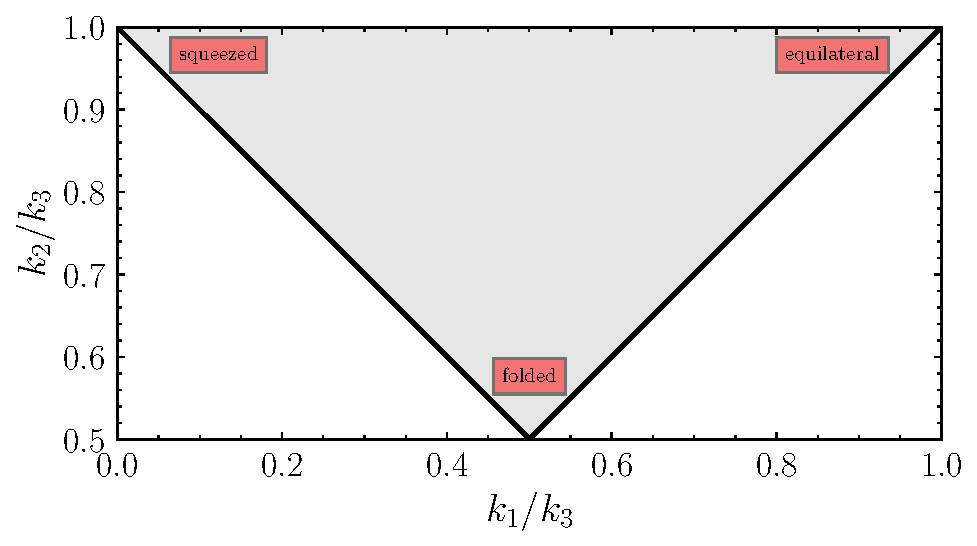
\includegraphics[width=0.8\textwidth]{region_plot.pdf}
\caption{Range of momenta $\cal V$ for plotting a shape function ${\cal S}(x_1,x_2,1)$, and for computing the cosine between two shapes. 
The \emph{equilateral} configuration is $x_1\to1,x_2\to 1$, while the \emph{squeezed} configuration is $x_1\to 0,x_2\to 1$, i.e.~it is 
the limit in which one of the modes ($k_1$) becomes much longer than the other two. 
The configuration $x_1\to1/2,x_2\to1/2$ is called \emph{folded}, and it corresponds to very squashed isosceles triangle.} 
\label{fig:region_plot}
\end{figure} 

We then define the equilateral shape as 
\begin{equation}
\boxed{{\cal S}_{\rm equil}(k_1,k_2,k_3) = \bigg(\frac{k_1}{k_2} + \text{$5$ perms.}\bigg) - \bigg(\frac{k_1^2}{k_2k_3} + \text{$2$ perms.}\bigg) - 2\,\,.} 
\end{equation}
The orthogonal shape can be defined as 
\begin{equation}
\boxed{{\cal S}_{\rm ortho}(k_1,k_2,k_3) = \frac{1}{{\cal N}_{\rm ortho}}\bigg[(1+p)\,\frac{\Delta}{e_3} - p\,\frac{\Gamma^3}{e_3^2}\bigg]\,\,,} 
\end{equation} 
\textbf{where} 
\begin{align*}
%\boxed{
p &= \frac{27}{\frac{743}{7(20\pi^2-193)} - 21}\,\,,%} 
\\
%\boxed{
\Delta &= (k_T-2k_1)(k_T-2k_2)(k_T-2k_3)\,\,,%} 
\\
%\boxed{
\Gamma &= \frac{2}{3}e_2 - \frac{1}{3}(k_1^2+k_2^2+k_3^2)\,\,,%} 
\\
%\boxed{
{\cal N}_{\rm ortho} &= \frac{840\pi^2 - 7363 - 189\,(20\pi^2-193)}{29114 - 2940\pi^2}\,\,.%} 
\end{align*}
${\cal S}_{\rm ortho}$ has the property that 
\begin{equation}
\frac{\braket{{\cal S}_{\rm equil}|{\cal S}_{\rm ortho}}}{\sqrt{\braket{{\cal S}_{\rm equil}|{\cal S}_{\rm equil}}\braket{{\cal S}_{\rm ortho}|{\cal S}_{\rm ortho}}}} = 0\,\,. 
\end{equation}
I checked this by computing the integral numerically: the overlap is zero for all practical purposes (which is quite amazing, I wonder how they found such shape). 
The other property is that in the squeezed limit ${\cal S}_{\rm ortho}$ behaves as expected. We can see this by the plots of Fig.~\ref{fig:equil_ortho}. 
\begin{figure}[h!]
\centering
\begin{tabular}{cc}
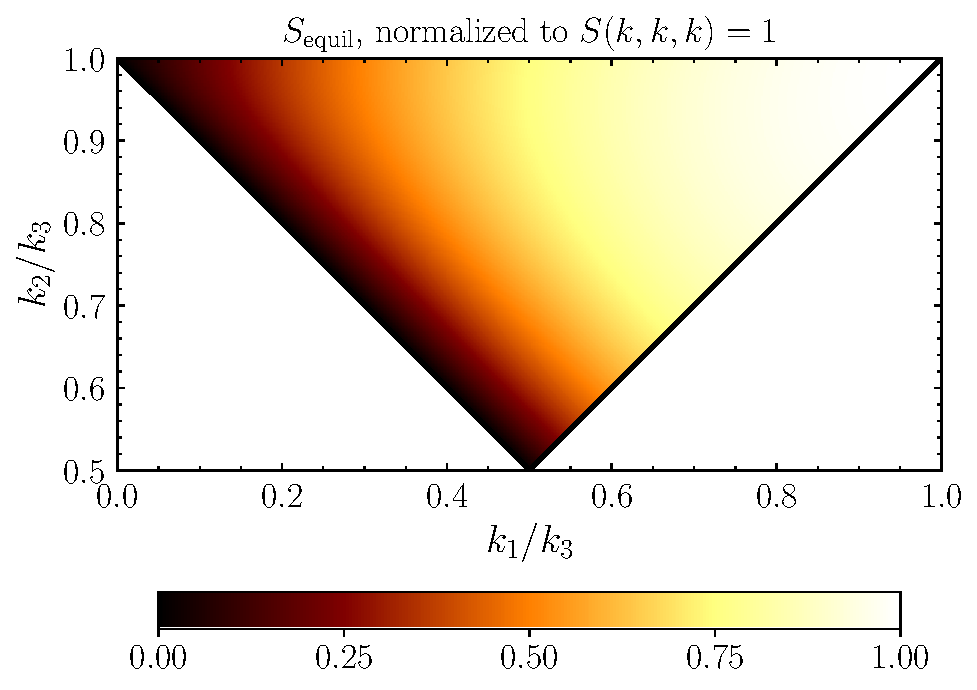
\includegraphics[width=0.475\columnwidth]{plot_equilateral.pdf} 
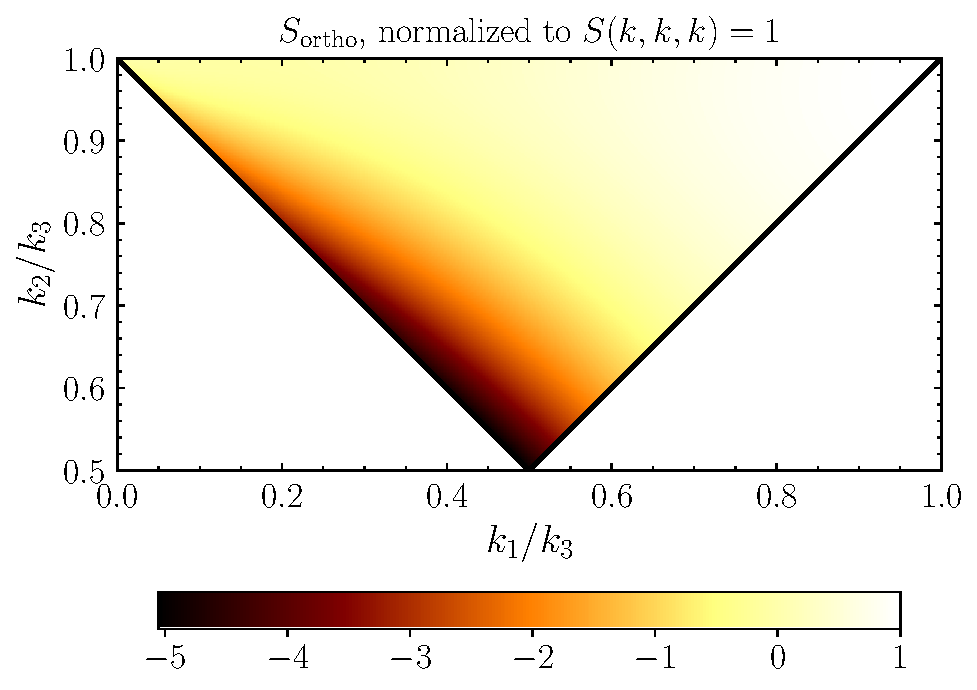
\includegraphics[width=0.475\columnwidth]{plot_orthogonal.pdf}
\end{tabular}
\caption{{Left panel} -- Equilateral shape, which also peaks in the equilateral configuration. 
{Right panel} -- Orthogonal shape: we see that it has the correct behavior in the equilateral and squeezed configurations.} 
\label{fig:equil_ortho}
\end{figure} 

Now, the idea is that we can put constraints on $f_{\rm NL}^{\rm equil}$ and $f_{\rm NL}^{\rm ortho}$. I.e., we take the primordial bispectrum to be given by 
\begin{equation}
\ket{S} = f_{\rm NL}^{\rm equil}\ket{S_{\rm equil}} + f_{\rm NL}^{\rm ortho}\ket{S_{\rm ortho}}\,\,. 
\end{equation} 
%and we constrain \emph{separately} $f_{\rm NL}^{\rm equil}$ and $f_{\rm NL}^{\rm ortho}$. 
The point is that the EFTI bispectrum is given by 
\begin{equation}
\ket{S} = f_{\rm NL}^{\dot{\pi}(\vec{\nabla}\pi)^2}\ket{S_{\dot{\pi}(\vec{\nabla}\pi)^2}} + f_{\rm NL}^{\dot{\pi}^3}\ket{S_{\dot{\pi}^3}}\,\,. 
\end{equation} 
Bra-ing $\ket{S}$ with $\bra{S_{\rm equil}}$ and $\bra{S_{\rm ortho}}$ and using that $\braket{{\cal S}_{\rm equil}|{\cal S}_{\rm ortho}}=0$, we find 
\begin{equation}
\boxed{\begin{pmatrix}
f_{\rm NL}^{\rm equil} \\
f_{\rm NL}^{\rm ortho}
\end{pmatrix}
 = {\underbrace{\begin{pmatrix}
\frac{\braket{{\cal S}_{\rm equil}|S_{\dot{\pi}(\vec{\nabla}\pi)^2}}}{\braket{{\cal S}_{\rm equil}|{\cal S}_{\rm equil}}} & \frac{\braket{{\cal S}_{\rm equil}|S_{\dot{\pi}^3}}}{\braket{{\cal S}_{\rm equil}|{\cal S}_{\rm equil}}} \\
\frac{\braket{{\cal S}_{\rm ortho}|S_{\dot{\pi}(\vec{\nabla}\pi)^2}}}{\braket{{\cal S}_{\rm ortho}|{\cal S}_{\rm ortho}}} & \frac{\braket{{\cal S}_{\rm ortho}|S_{\dot{\pi}^3}}}{\braket{{\cal S}_{\rm ortho}|{\cal S}_{\rm ortho}}}
\end{pmatrix}}_{{M}^{-1}}}
\begin{pmatrix}
f_{\rm NL}^{\dot{\pi}(\vec{\nabla}\pi)^2} \\
f_{\rm NL}^{\dot{\pi}^3}
\end{pmatrix}\,\,.} 
\end{equation} 
Hence, we can define 
\begin{equation}
\begin{pmatrix}
f_{\rm NL}^{\rm equil} \\
f_{\rm NL}^{\rm ortho}
\end{pmatrix}_{\dot{\pi}(\vec{\nabla}\pi)^2}
 = \begin{pmatrix}
\frac{\braket{{\cal S}_{\rm equil}|S_{\dot{\pi}(\vec{\nabla}\pi)^2}}}{\braket{{\cal S}_{\rm equil}|{\cal S}_{\rm equil}}} & \frac{\braket{{\cal S}_{\rm equil}|S_{\dot{\pi}^3}}}{\braket{{\cal S}_{\rm equil}|{\cal S}_{\rm equil}}} \\
\frac{\braket{{\cal S}_{\rm ortho}|S_{\dot{\pi}(\vec{\nabla}\pi)^2}}}{\braket{{\cal S}_{\rm ortho}|{\cal S}_{\rm ortho}}} & \frac{\braket{{\cal S}_{\rm ortho}|S_{\dot{\pi}^3}}}{\braket{{\cal S}_{\rm ortho}|{\cal S}_{\rm ortho}}}
\end{pmatrix}
\begin{pmatrix}
1 \\
0
\end{pmatrix} %\,\,,
\end{equation} 
and 
\begin{equation}
\begin{pmatrix}
f_{\rm NL}^{\rm equil} \\
f_{\rm NL}^{\rm ortho}
\end{pmatrix}_{\dot{\pi}^3}
 = \begin{pmatrix}
\frac{\braket{{\cal S}_{\rm equil}|S_{\dot{\pi}(\vec{\nabla}\pi)^2}}}{\braket{{\cal S}_{\rm equil}|{\cal S}_{\rm equil}}} & \frac{\braket{{\cal S}_{\rm equil}|S_{\dot{\pi}^3}}}{\braket{{\cal S}_{\rm equil}|{\cal S}_{\rm equil}}} \\
\frac{\braket{{\cal S}_{\rm ortho}|S_{\dot{\pi}(\vec{\nabla}\pi)^2}}}{\braket{{\cal S}_{\rm ortho}|{\cal S}_{\rm ortho}}} & \frac{\braket{{\cal S}_{\rm ortho}|S_{\dot{\pi}^3}}}{\braket{{\cal S}_{\rm ortho}|{\cal S}_{\rm ortho}}}
\end{pmatrix}
\begin{pmatrix}
0 \\
1
\end{pmatrix}\,\,.
\end{equation} 
I.e., taking 
\begin{equation}
\ket{S} = (f_{\rm NL}^{\rm equil})_{\dot{\pi}(\vec{\nabla}\pi)^2}\ket{S_{\rm equil}} + (f_{\rm NL}^{\rm ortho})_{\dot{\pi}(\vec{\nabla}\pi)^2}\ket{S_{\rm ortho}} %\,\,. 
\end{equation} 
should reproduce $f_{\rm NL}^{\dot{\pi}(\vec{\nabla}\pi)^2} = 1$ and $f_{\rm NL}^{\dot{\pi}^3}=0$, and vice-versa for the other choice. 
In practice, the resulting ${\dot{\pi}(\vec{\nabla}\pi)^2}$ shape is essentially indistinguishable from the true EFTI one. 
It has a cosine with it equal to $1$, it has a normalization at $(k,k,k)$ equal to $1.0007$ (which one can re-normalize anyway), and its two-dimensional plot is indistinguishable by eye. The plot is shown in Fig.~\ref{fig:dotpinablapisquared}. 
\begin{figure}[h!]
\centering
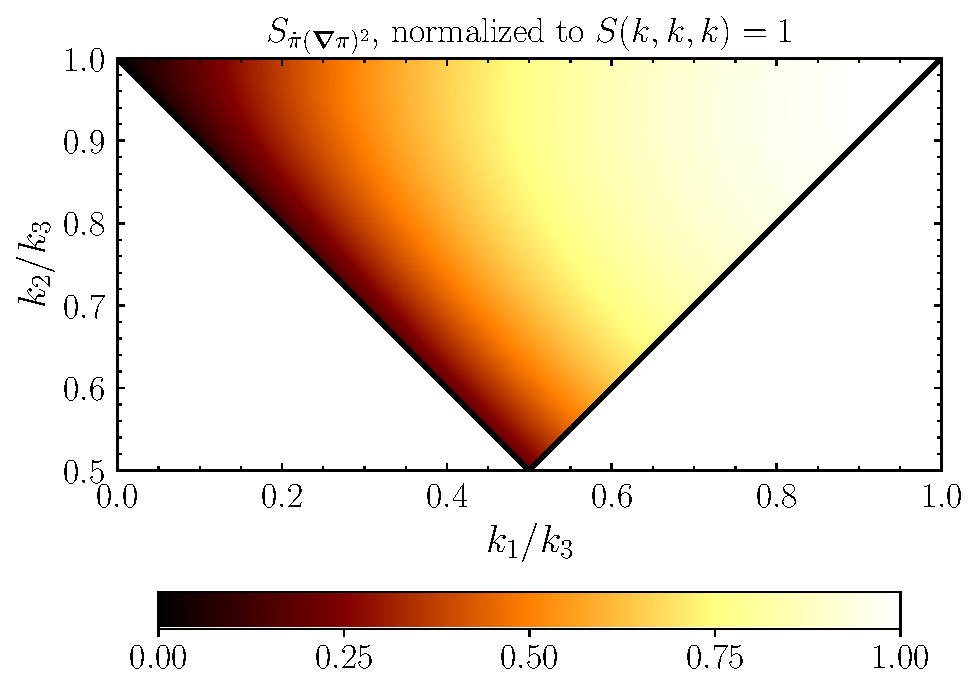
\includegraphics[width=0.8\textwidth]{plot_dotpinablapisquared.pdf}
\caption{Plot of the EFTI shape from $\dot{\pi}(\vec{\nabla}\pi)^2$. This is indistinguishable by eye from the one constructed by combining equilateral and orthogonal shapes.} 
\label{fig:dotpinablapisquared}
\end{figure} 

For the $\dot{\pi}^3$ shape, the cosine with the EFTI one is very close to one: it is $0.9995$. However, we notice that its normalization is $1.035$.\footnote{Here I do not mean its norm with respect to the dot product! I mean the normalization at $(k,k,k)$, which has nothing to do with it. The norm is preserved via the usual bra-ket formulas, using that $\braket{{\cal S}_{\rm equil}|{\cal S}_{\rm ortho}}=0$.} So one should re-normalize it in principle (given the large uncertainties in the determination of these from data, this is irrelevant I think). The two-dimensional plot showing the difference (in which I re-normalized the ``mock'' $\dot{\pi}^3$ shape), is in Fig.~\ref{fig:dotpicubed_comparison}. 
\begin{figure}[h!]
\centering
\begin{tabular}{cc}
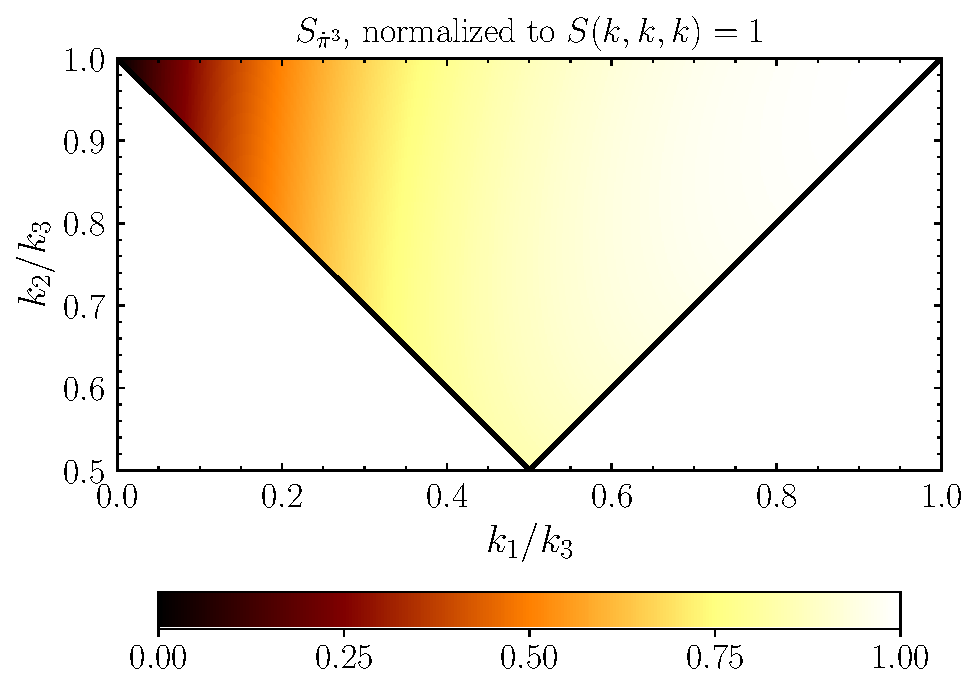
\includegraphics[width=0.475\columnwidth]{plot_dotpicubed.pdf} 
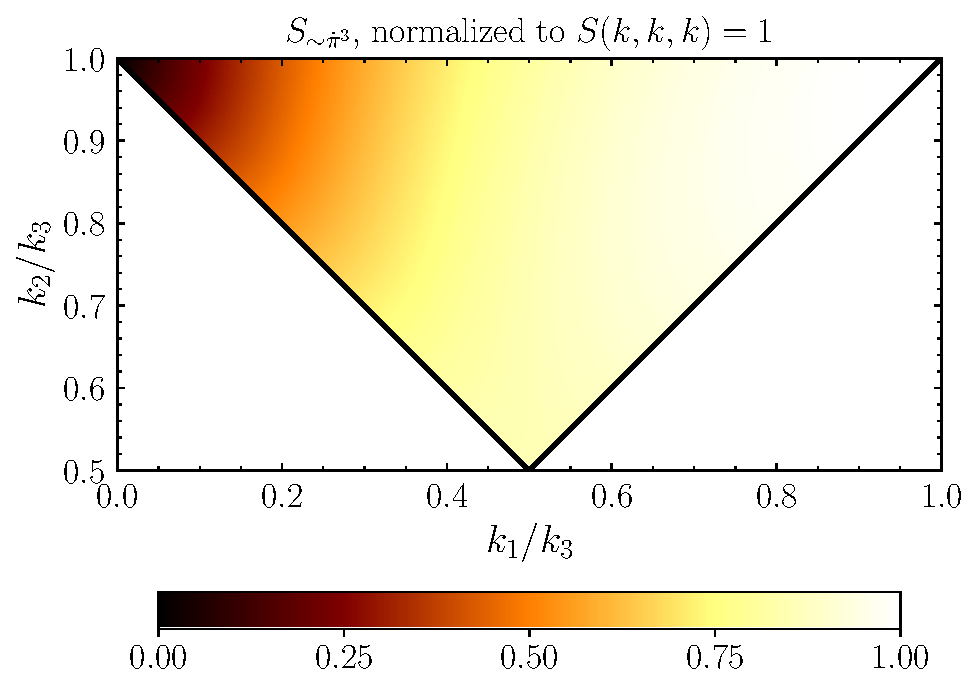
\includegraphics[width=0.475\columnwidth]{plot_dotpicubedcombo.pdf}
\end{tabular}
\caption{{Left panel} -- EFTI shape from $\dot{\pi}^3$. 
{Right panel} -- Its approximation by equilateral and orthogonal shapes.} 
\label{fig:dotpicubed_comparison}
\end{figure} 


%********************************************************
\section{What this all means}
\label{sec:what_this_means} 
%********************************************************


\noindent I see it this way. We want to constrain 
\begin{equation}
\ket{S} = f_{\rm NL}^{\dot{\pi}(\vec{\nabla}\pi)^2}\ket{S_{\dot{\pi}(\vec{\nabla}\pi)^2}} + f_{\rm NL}^{\dot{\pi}^3}\ket{S_{\dot{\pi}^3}}\,\,. 
\end{equation} 
Then, we should constrain 
\begin{equation}
\ket{S} = f_{\rm NL}^{\rm equil}\ket{S_{\rm equil}} + f_{\rm NL}^{\rm ortho}\ket{S_{\rm ortho}}%\,\,. 
\end{equation} 
with BOTH shapes at the same time. Find a two-dimensional contour for $f_{\rm NL}^{\rm equil}$ and $f_{\rm NL}^{\rm ortho}$, and then translate it 
to $f_{\rm NL}^{\dot{\pi}(\vec{\nabla}\pi)^2}$ and $f_{\rm NL}^{\dot{\pi}^3}$ via the matrix discussed in the previous section. 

In other words, it does not make much sense to constrain the orthogonal shape \emph{by itself}, in my understanding. Is this why Matias does not like it? 
In any case: maybe we can argue the following. Given that $\braket{{\cal S}_{\rm equil}|{\cal S}_{\rm ortho}}=0$, maybe we can argue that $f_{\rm NL}^{\rm ortho}\ket{S_{\rm equil}}$ and $f_{\rm NL}^{\rm ortho}\ket{S_{\rm ortho}}$ are not degenerate, so we can constrain them separately, and then make a non-degenerate two-dimensional Gaussian out of their marginalized one-dimensional constraints, and apply to it the matrix? 

An alternative is noticing, by comparing Fig.~\ref{fig:dotpinablapisquared} with the left panel of Fig.~\ref{fig:equil_ortho}, that the equilateral shape is already very very similar to $\dot{\pi}(\vec{\nabla}\pi)^2$. Indeed, notice that 
\begin{equation}
\frac{\braket{{\cal S}_{\rm equil}|{\cal S}_{\rm ortho}}}{\sqrt{\braket{{\cal S}_{\rm equil}|{\cal S}_{\rm equil}}\braket{{\cal S}_{\rm ortho}|{\cal S}_{\rm ortho}}}} = 0.997\,\,. 
\end{equation} 
\emph{In other words, the matrix $M^{-1}$ of the previous section can be very well approximated by an upper-triangular matrix!} Indeed, it is 
%--> notice that Misha is right that the overlap and cosine here is studied WITHOUT cosmic variance or instrumental noise, and including ALL MODES. This is fine for the "deterministic" formulas to relate the f_{NL} of templates to those of operators. If I had a perfect determination of the former, I would get a perfect determination for the latter. Now, instead, I have an error on the former, and then this translates to an error on the latter via this formula... 
\begin{equation}
%{{1.04021, 1.21041}, {-0.0395140, -0.175685}}
M^{-1} = \begin{pmatrix}
%1.04 & 1.21 \\
%-0.04 & -0.18
1.04021 & 1.21041 \\
-0.0395140 & -0.175685
\end{pmatrix}
\,\,. 
\end{equation}
Hence one could constrain the equilateral shape as we are now doing, and:
\begin{itemize}[leftmargin=*]
\item either use directly the non-separable shape for ${\dot\pi}^3$, which is why I was thinking at the beginning; 
\item just use the linear combination of the right panel of Fig.~\ref{fig:dotpicubed_comparison} as a replacement for it. 
\end{itemize}
\textbf{This alternative, with the latter point, is the cheapest and quickest way.} We should discuss. But notice that most likely Leonardo will complain because these two shapes are assumed to be there BOTH at the same time in the EFTI. While I can argue that in the small-speed-of-sound case the one with spatial derivatives is the leading one, can I argue that there is a situation where only the $(g^{00}+1)^3$ operator is turned on, or is leading? Unlikely. But for now, I think it is fair to do it separately and just mention this, and say that we plan to do a more detailed analysis going back to this when we include local NG. 


%********************************************************
\section{What we decided, and EFTI}
\label{sec:what_we_decided_and_EFTI} 
%********************************************************


\noindent \textbf{We decided to constrain both equilateral and orthogonal, and to constrain the EFTI.} 
Let us see in more detail what this is. Recall we have 
\begin{equation}
\boxed{\begin{pmatrix}
f_{\rm NL}^{\rm equil} \\
f_{\rm NL}^{\rm ortho}
\end{pmatrix}
 = {\underbrace{\begin{pmatrix}
\frac{\braket{{\cal S}_{\rm equil}|S_{\dot{\pi}(\vec{\nabla}\pi)^2}}}{\braket{{\cal S}_{\rm equil}|{\cal S}_{\rm equil}}} & \frac{\braket{{\cal S}_{\rm equil}|S_{\dot{\pi}^3}}}{\braket{{\cal S}_{\rm equil}|{\cal S}_{\rm equil}}} \\
\frac{\braket{{\cal S}_{\rm ortho}|S_{\dot{\pi}(\vec{\nabla}\pi)^2}}}{\braket{{\cal S}_{\rm ortho}|{\cal S}_{\rm ortho}}} & \frac{\braket{{\cal S}_{\rm ortho}|S_{\dot{\pi}^3}}}{\braket{{\cal S}_{\rm ortho}|{\cal S}_{\rm ortho}}}
\end{pmatrix}}_{{M}^{-1}}}
\begin{pmatrix}
f_{\rm NL}^{\dot{\pi}(\vec{\nabla}\pi)^2} \\
f_{\rm NL}^{\dot{\pi}^3}
\end{pmatrix}\,\,,} 
\end{equation} 
where 
\begin{equation}
%{{1.04021, 1.21041}, {-0.0395140, -0.175685}}
M^{-1} = \begin{pmatrix}
%1.04 & 1.21 \\
%-0.04 & -0.18
1.04021 & 1.21041 \\
-0.0395140 & -0.175685
\end{pmatrix}
\,\,. 
\end{equation}

This equation holds at the level of the shapes. Now, the data tell us the constraints on $f_{\rm NL}^{\rm equil}$ and $f_{\rm NL}^{\rm ortho}$ 
(which do not need to be completely uncorrelated, since $f_{\rm NL}^{\rm equil}$ and $f_{\rm NL}^{\rm ortho}$ are orthogonal only at the ``theory level''). 
From this we obtain constraints on $f_{\rm NL}^{\dot{\pi}(\vec{\nabla}\pi)^2}$ and $f_{\rm NL}^{\dot{\pi}^3}$ via 
\begin{equation}
\begin{pmatrix}
f_{\rm NL}^{\dot{\pi}(\vec{\nabla}\pi)^2} \\
f_{\rm NL}^{\dot{\pi}^3}
\end{pmatrix} 
= M
\begin{pmatrix}
f_{\rm NL}^{\rm equil} \\
f_{\rm NL}^{\rm ortho}
\end{pmatrix}
\,\,. 
\end{equation} 
Then, we want to relate $f_{\rm NL}^{\dot{\pi}(\vec{\nabla}\pi)^2}$ and $f_{\rm NL}^{\dot{\pi}^3}$ to the EFTI Lagrangian. This is 
\begin{equation}
\begin{split} 
S &= \int\dif^4x\,\sqrt{-g}\,\bigg[\frac{\mpl^2}{2}R - c(t)g^{00} - \Lambda(t) + \frac{M_2^4(t)}{2}\,(g^{00}+1)^2 + \frac{M_3^4(t)}{6}\,(g^{00}+1)^3 \\ 
&\hp{= \int\dif^4x\,\sqrt{-g}\,\bigg[}\,\, - \frac{\bar{M}^3_1(t)}{2}\,(g^{00}+1)\,\delta\!K^\mu_{\hp{\mu}\mu} 
- \frac{\bar{M}^2_2(t)}{2}\,(\delta\!K^\mu_{\hp{\mu}\mu})^2 + \cdots\bigg]\,\,. 
\end{split} 
\end{equation} 
In the decoupling limit and with the approximation of constant coefficients this becomes 
\begin{equation}
\begin{split}
S_\pi &= \int\dif^4x\,a^3\Bigg[{-\mpl^2}\dot{H}\bigg(\dot{\pi}^2 - \frac{\vec{\nabla}\pi\!\cdot\! 
\vec{\nabla}\pi}{a^2}\bigg) + 2M^4_2\bigg(\dot{\pi}^2 + \dot{\pi}^3 - \dot{\pi}\frac{\vec{\nabla}\pi\!\cdot\! 
\vec{\nabla}\pi}{a^2}\bigg) - \frac{4}{3}M^4_3\dot{\pi}^3 + \cdots\bigg] %\\
%%&\hp{= \int\dif^4x\,a^3\bigg[}\,\, \\ 
%&\hp{= \int\dif^4x\,a^3\bigg[}\,\, - \frac{\bar{M}^2_2}{2}\bigg\{(1 - 2\dot{\pi})\frac{(\nabla^2\pi)^2}{a^4} 
%- \frac{\nabla^2\pi}{a^2}\bigg(\frac{H\vec{\nabla}\pi\!\cdot\!\vec{\nabla}\pi}{a^2} 
%+ \frac{4\vec{\nabla}\pi\!\cdot\!\vec{\nabla}\dot{\pi}}{a^2}\bigg) + \cdots\bigg\}\Bigg]
\,\,, 
\end{split}
\end{equation} 
where for now I neglect all the operators beyond $P(X)$, i.e.~beyond $(g^{00}+1)^n$. 
If we want to translate our constraints on the Ghost Condensate we will do it later. 
From this equation we see that the quadratic action is 
\begin{equation}
\int\dif^4x\,a^3\bigg[{-\frac{\mpl^2\dot{H}}{c^2_{\rm s}}}\bigg(\dot{\pi}^2 - c^2_{\rm s}\frac{\vec{\nabla}\pi\!\cdot\! 
\vec{\nabla}\pi}{a^2}\bigg)\bigg]\,\,, 
\end{equation} 
with speed of sound given by 
\begin{equation} 
\frac{1}{c^2_{\rm s}} = 1-\frac{2M^4_2}{\dot{H}\mpl^2}\Rightarrow \frac{2M^4_2}{\dot{H}\mpl^2} = \frac{c^2_{\rm s}-1}{c^2_{\rm s}} \Rightarrow {-2M^4_2} = {\dot{H}\mpl^2}\frac{1-c^2_{\rm s}}{c^2_{\rm s}}\,\,. 
\end{equation} 
Then, we see that the cubic action is 
\begin{equation}
\begin{split} 
S^{(3)}_\pi &= \int\dif^4x\,a^3\bigg[%{-\frac{\mpl^2\dot{H}}{c^2_{\rm s}}}
2M^4_2\bigg(\dot{\pi}^3 - \dot{\pi}\frac{\vec{\nabla}\pi\!\cdot\! 
\vec{\nabla}\pi}{a^2}\bigg) - \frac{4}{3}M^4_3\dot{\pi}^3\bigg] \\ 
&= \int\dif^4x\,a^3\bigg[{-2M^4_2}\,{\cal O}_{\dot{\pi}(\vec{\nabla}\pi)^2} + \bigg(2M^4_2 - \frac{4}{3}M^4_3\bigg){\cal O}_{\dot{\pi}^3}\bigg]\,\,, 
\end{split} 
\end{equation}
where the definition of ${\cal O}_{\dot{\pi}(\vec{\nabla}\pi)^2}$ and ${\cal O}_{\dot{\pi}^3}$ is straightforward. Then, the Lagrangian becomes 
\begin{equation}
\begin{split} 
S^{(3)}_\pi &= {\dot{H}\mpl^2}\int\dif^4x\,a^3\bigg[\frac{1-c^2_{\rm s}}{c^2_{\rm s}}\,{\cal O}_{\dot{\pi}(\vec{\nabla}\pi)^2} - \bigg(\frac{1-c^2_{\rm s}}{c^2_{\rm s}} + \frac{4}{3}\frac{M^4_3}{{\dot{H}\mpl^2}}\bigg){\cal O}_{\dot{\pi}^3}\bigg]\,\,. 
\end{split} 
\end{equation} 
If we define 
\begin{equation}
\frac{4}{3}\frac{M^4_3}{{\dot{H}\mpl^2}} = \frac{2}{3} \frac{1-c^2_{\rm s}}{c^2_{\rm s}} \frac{\tilde{c}_3}{c^2_{\rm s}} %\,\,,
\end{equation} 
we match Leonardo's definitions in Eq.~(8) of the WMAP paper, since we have 
\begin{equation}
\begin{split} 
S^{(3)}_\pi &= {\dot{H}\mpl^2}\frac{1-c^2_{\rm s}}{c^2_{\rm s}}\int\dif^4x\,a^3\bigg[%\frac{1-c^2_{\rm s}}{c^2_{\rm s}}\,
{\cal O}_{\dot{\pi}(\vec{\nabla}\pi)^2} - \bigg(1 + \frac{2}{3}\frac{\tilde{c}_3}{c^2_{\rm s}}\bigg){\cal O}_{\dot{\pi}^3}\bigg]\,\,. 
\end{split} 
\end{equation} 
Other definitions can be found in \url{https://arxiv.org/abs/0709.0295}. Eqs.~(33) and (34) of that paper say that what there is called $c_3$, here is called $\tilde{c}_3/c^2_{\rm s}$. 

Leonardo comments on the UV/unitarity cutoff from these two operators. One finds (recall that $\dot{H}$ is negative) 
\begin{align}
\Lambda^4_{\dot{\pi}(\vec{\nabla}\pi)^2} &= -16\pi^2\dot{H}\mpl^2\frac{c^5_{\rm s}}{(1-c^2_{\rm s})^2}\,\,, \\
\Lambda^4_{\dot{\pi}^3} &= \frac{\Lambda^4_{\dot{\pi}(\vec{\nabla}\pi)^2}}{(c^2_{\rm s} + \frac{2\tilde{c}_3}{3})^2}\,\,.
\end{align}
We see that for $\tilde{c}_3 = 0$, the correct scaling due to having less spatial derivatives is respected. So putting constraints on the size of these operators constrains these scales, which was the original dream I guess. 

What else? We actually need to write down the relation of $c^2_{\rm s}$ and $\tilde{c}_3$ to 
$f_{\rm NL}^{\dot{\pi}(\vec{\nabla}\pi)^2}$ and $f_{\rm NL}^{\dot{\pi}^3}$. Let us first work it out from Leonardo's WMAP paper, 
and then I will recompute the $\pi$ (and hence $\zeta$) correlators myself.\footnote{This check is not detailed in these notes.} 
We have that he writes 
\begin{equation}
B_\phi^{\dot{\pi}(\vec{\nabla}\pi)^2}(k_1,k_2,k_3) = \bigg(\frac{3}{5}\bigg)^3B_\zeta^{\dot{\pi}(\vec{\nabla}\pi)^2}(k_1,k_2,k_3) = \frac{5}{12}\frac{1-c^2_{\rm s}}{c^2_{\rm s}}\Delta^4_\phi 
\frac{24e_3^2-8e_2e_3k_T-8e_2^2k_T^2+22e_3k_T^3-6e_2k_T^4+2k_T^6}{k_T^3 e_3^3}\,\,, 
\end{equation}
where 
\begin{equation}
\Delta^2_\phi = \bigg(\frac{3}{5}\bigg)^2\Delta^2_\zeta\,\,. 
\end{equation}
Hence we find 
\begin{equation}
\begin{split}
B_\zeta^{\dot{\pi}(\vec{\nabla}\pi)^2}(k_1,k_2,k_3) &= \bigg(\frac{3}{5}\bigg)^{-3} \frac{5}{12}\frac{1-c^2_{\rm s}}{c^2_{\rm s}}\bigg(\frac{3}{5}\bigg)^4\Delta^4_\zeta 
\frac{24e_3^2-8e_2e_3k_T-8e_2^2k_T^2+22e_3k_T^3-6e_2k_T^4+2k_T^6}{k_T^3 e_3^3} \\
&=\frac{1}{4}\frac{1-c^2_{\rm s}}{c^2_{\rm s}} \Delta^4_\zeta 
\frac{24e_3^2-8e_2e_3k_T-8e_2^2k_T^2+22e_3k_T^3-6e_2k_T^4+2k_T^6}{k_T^3 e_3^3}\,\,. 
\end{split}
\end{equation}
From this we get 
\begin{equation}
f_{\rm NL}^{\dot{\pi}(\vec{\nabla}\pi)^2} {\cal S}^{\dot{\pi}(\vec{\nabla}\pi)^2}(k_1,k_2,k_3) = \frac{5}{72}\frac{1-c^2_{\rm s}}{c^2_{\rm s}} 
\frac{24e_3^2-8e_2e_3k_T-8e_2^2k_T^2+22e_3k_T^3-6e_2k_T^4+2k_T^6}{k_T^3 e_3}\,\,. 
\end{equation} 
Multiplying and dividing by ${\cal N}_{\dot{\pi}(\vec{\nabla}\pi)^2}$, we get 
\begin{equation}
f_{\rm NL}^{\dot{\pi}(\vec{\nabla}\pi)^2} {\cal S}^{\dot{\pi}(\vec{\nabla}\pi)^2}(k_1,k_2,k_3) = \frac{5}{72}{\cal N}_{\dot{\pi}(\vec{\nabla}\pi)^2}\frac{1-c^2_{\rm s}}{c^2_{\rm s}}{\underbrace{\bigg[\frac{1}{{\cal N}_{\dot{\pi}(\vec{\nabla}\pi)^2}} 
\frac{24e_3^2-8e_2e_3k_T-8e_2^2k_T^2+22e_3k_T^3-6e_2k_T^4+2k_T^6}{k_T^3 e_3}\bigg]}_{\hphantom{{\cal S}^{\dot{\pi}(\vec{\nabla}\pi)^2}(k_1,k_2,k_3)\,}=\,{\cal S}^{\dot{\pi}(\vec{\nabla}\pi)^2}(k_1,k_2,k_3)}}\,\,. 
\end{equation} 
This tells us that 
\begin{equation}
\boxed{f_{\rm NL}^{\dot{\pi}(\vec{\nabla}\pi)^2} = \frac{5}{72}{\cal N}_{\dot{\pi}(\vec{\nabla}\pi)^2}\frac{1-c^2_{\rm s}}{c^2_{\rm s}} = 
{-\frac{34}{9}}\frac{5}{72}\frac{1-c^2_{\rm s}}{c^2_{\rm s}} = {-\frac{85}{324}}\frac{1-c^2_{\rm s}}{c^2_{\rm s}} = \frac{85}{324}\bigg(1-\frac{1}{c^2_{\rm s}}\bigg)\,\,.} 
\end{equation} 

Let us then go to the other operator. We have 
\begin{equation}
B_\phi^{\dot{\pi}^3}(k_1,k_2,k_3) = \bigg(\frac{3}{5}\bigg)^3B_\zeta^{\dot{\pi}^3}(k_1,k_2,k_3) = {-\frac{20}{3}}\frac{1-c^2_{\rm s}}{c^2_{\rm s}}\bigg(\tilde{c}_3+\frac{3}{2}c^2_{\rm s}\bigg)\Delta^4_\phi\frac{1}{k_T^3e_3}\,\,. 
\end{equation}
Hence we get 
\begin{equation}
B_\zeta^{\dot{\pi}^3}(k_1,k_2,k_3) = \bigg(\frac{3}{5}\bigg)^{-3}\bigg({-\frac{20}{3}}\bigg)\frac{1-c^2_{\rm s}}{c^2_{\rm s}}\bigg(\tilde{c}_3+\frac{3}{2}c^2_{\rm s}\bigg)\bigg(\frac{3}{5}\bigg)^{4}\Delta^4_\zeta\frac{1}{k_T^3e_3} = {-4}\frac{1-c^2_{\rm s}}{c^2_{\rm s}}\bigg(\tilde{c}_3+\frac{3}{2}c^2_{\rm s}\bigg)\Delta^4_\zeta\frac{1}{k_T^3e_3}\,\,. 
\end{equation} 
Hence, we get 
\begin{equation}
f_{\rm NL}^{\dot{\pi}^3} {\cal S}^{\dot{\pi}^3}(k_1,k_2,k_3) = {-\frac{10}{9}}\frac{1-c^2_{\rm s}}{c^2_{\rm s}}\bigg(\tilde{c}_3+\frac{3}{2}c^2_{\rm s}\bigg) \frac{e_3}{k_T^3} \,\,. 
\end{equation} 
Multiplying and dividing by ${\cal N}_{\dot{\pi}^3}$, we get 
\begin{equation}
f_{\rm NL}^{\dot{\pi}^3} {\cal S}^{\dot{\pi}^3}(k_1,k_2,k_3) = {-\frac{10}{9}}{\cal N}_{\dot{\pi}^3}\frac{1-c^2_{\rm s}}{c^2_{\rm s}}\bigg(\tilde{c}_3+\frac{3}{2}c^2_{\rm s}\bigg) {\underbrace{\bigg[\frac{1}{{\cal N}_{\dot{\pi}^3}}\frac{e_3}{k_T^3}\bigg]}_{{\cal S}^{\dot{\pi}^3}(k_1,k_2,k_3)}}\,\,. 
\end{equation} 
This tells us that 
\begin{equation}
\boxed{f_{\rm NL}^{\dot{\pi}^3} = {-\frac{10}{9}}{\cal N}_{\dot{\pi}^3}\frac{1-c^2_{\rm s}}{c^2_{\rm s}}\bigg(\tilde{c}_3+\frac{3}{2}c^2_{\rm s}\bigg) = 
{-\frac{10}{243}}\frac{1-c^2_{\rm s}}{c^2_{\rm s}}\bigg(\tilde{c}_3+\frac{3}{2}c^2_{\rm s}\bigg) = 
{\frac{10}{243}}\bigg(1-\frac{1}{c^2_{\rm s}}\bigg)\bigg(\tilde{c}_3+\frac{3}{2}c^2_{\rm s}\bigg)\,\,.} 
\end{equation} 

Then, we have the formulas. Leonardo and \emph{Planck} put constraints in the plane $c_{\rm s}$ -- $\tilde{c}_3(1/c^2_{\rm s}-1)$ (notice, the $x$ axis is not $c^2_{\rm s}$). 
Let us call 
\begin{equation}
\tilde{c}_3\bigg(\frac{1}{c^2_{\rm s}}-1\bigg) = \tilde{c}_3\bigg(\frac{1-c^2_{\rm s}}{c^2_{\rm s}}\bigg) \equiv y_{\rm LEO}\,\,. 
\end{equation} 
We have 
\begin{equation}
\begin{pmatrix}
f_{\rm NL}^{\dot{\pi}(\vec{\nabla}\pi)^2} \\
f_{\rm NL}^{\dot{\pi}^3}
\end{pmatrix} 
= M
\begin{pmatrix}
f_{\rm NL}^{\rm equil} \\
f_{\rm NL}^{\rm ortho}
\end{pmatrix}
\,\,, 
\end{equation} 
where the matrix $M$ is defined above (or better, $M^{-1}$ is). First, we then write 
\begin{equation}
f_{\rm NL}^{\dot{\pi}^3} = 
{-\frac{10}{243}}\frac{1-c^2_{\rm s}}{c^2_{\rm s}}\bigg(\tilde{c}_3+\frac{3}{2}c^2_{\rm s}\bigg) = 
{-\frac{10}{243}}\frac{1-c^2_{\rm s}}{c^2_{\rm s}}\tilde{c}_3 - {\frac{5}{81}}({1-c^2_{\rm s}})
= {-\frac{10}{243}}y_{\rm LEO} - {\frac{5}{81}}({1-c^2_{\rm s}})\,\,. 
\end{equation} 
Then, we find 
\begin{equation}
\boxed{c^2_{\rm s} = \frac{1}{1-\frac{324}{85}f_{\rm NL}^{\dot{\pi}(\vec{\nabla}\pi)^2}}\,\,,}
\end{equation}
and 
\begin{equation}
\boxed{y_{\rm LEO} = \frac{243\Big[20f_{\rm NL}^{\dot{\pi}(\vec{\nabla}\pi)^2}+f_{\rm NL}^{\dot{\pi}^3}\big({-85} + 324f_{\rm NL}^{\dot{\pi}(\vec{\nabla}\pi)^2}\big)\Big]}{850 - 3240f_{\rm NL}^{\dot{\pi}(\vec{\nabla}\pi)^2}}\,\,.}
\end{equation} 
Notice that for large enough positive values of $f_{\rm NL}^{\dot{\pi}(\vec{\nabla}\pi)^2}$, which essentially are values of $f_{\rm NL}^{\rm equil}$ 
as discussed in previous sections, I risk to have a small and negative $c^2_{\rm s}$. In this case, higher-derivative terms must come in, etc.~etc.~I fear we need 
to discuss this if we really want to put constraints on the EFTI action? I fear that we will surely end up with allowing negative $c^2_{\rm s}$. 
Can we maybe work around by imposing a theoretical prior when we do the analysis in the $f_{\rm NL}^{\rm equil}$ and $f_{\rm NL}^{\rm ortho}$ variables, if we only want to consider $P(X)$?\footnote{Notice the conjecture that also says that $\tilde{c}_3$ is positive. Should ask Paolo about this.} 


%********************************************************
\section{Section 2 of paper}
\label{sec:sec_2_of_paper} 
%********************************************************


\noindent %At leading order in the expansion in ${-\dot{H}/H^2}$, which controls how close inflation is to a purely de Sitter expansion, 
For the large level of non-Gaussianities allowed by current data, the action for $\pi$ takes the universal form [EFTI] 
%--> check I copied correctly: check signs!!! 
\be
\label{eq:EFTI_action} 
{-\frac{\mpl^2\dot{H}}{c^2_{\rm s}}}\int\dif^4x\,a^3\bigg[\dot{\pi}^2 - c^2_{\rm s}\frac{(\vec{\nabla}\pi)^2}{a^2} 
- ({1-c^2_{\rm s}})\,\dot{\pi}\frac{(\vec{\nabla}\pi)^2}{a^2} + ({1-c^2_{\rm s}})\bigg(1 + \frac{2}{3}\frac{\tilde{c}_3}{c^2_{\rm s}}\bigg)\dot{\pi}^3\bigg]+ \dots\,\,, 
\ee
and $\pi$ is related to the curvature perturbation $\cal R$ by ${\cal R} = {-H\pi}$. 
[GIOVANNI: actually check again. Should we use $\zeta$, as \emph{Planck} and Leonardo? That would be great.] 
%The $\dots$ denote terms that are higher order in an expansion in $H/M$, where $M$ is some [\dots] 
The dots denote quadratic and cubic operators that are subleading unless %${-\dot{H}/H^2}$ is too small, or suppressed by $H/M$, where [...] 
one approaches the near de Sitter limit [GHOST\_INFLATION]. 
A class of microphysical models that realize this action are the so-called $P(X,\phi)$ Lagrangians for a scalar field $\phi$, where 
$X = -g^{\mu\nu}\partial_\mu\phi\partial_\nu\phi$. Chief among them is ``DBI Inflation'' [DBI], where $\phi$ is the position of a probe brane in a $5$-dimensional spacetime. 

Eq.~\eqref{eq:EFTI_action} tells us that the cubic action for $\pi$ is not controlled only by $c^2_{\rm s}$. 
The coefficient of the operator ${\dot\pi}^3$ depends also on the dimensionless parameter $\tilde{c}_3$: 
for general $P(X,\phi)$ models the speed of sound %$c_{\rm s}$ 
and %the dimensionless parameter 
$\tilde{c}_3$ are unrelated, 
while for DBI Inflation the relation $\tilde{c}_3 = 3({1-c^2_{\rm s}})/2$ is protected by the higher-dimensional Lorentz symmetry. 
Ref.~[SSZ\_WMAP] showed how the bispectrum shapes generated by the operators $\dot{\pi}(\vec{\nabla}\pi)^2$ and $\dot{\pi}^3$ can be captured 
by linear combinations of two \emph{templates}: the so-called \emph{equilateral} and \emph{orthogonal} templates $B_{\cal R}^{\rm equil}$ and $B_{\cal R}^{\rm ortho}$. These have the following properties: 
\begin{itemize}[leftmargin=*]
\item both templates vanish in the squeezed configuration, as is required if they need reproduce to single-field bispectra. 
\item they are separable in $k_1,k_2,k_3$; 
\item they achieve their maximum value in different configurations (the equilateral peaks for $k_1\approx k_2\approx k_3$, while the orthogonal peaks at ``folded'' triangles $k_1\approx k_2\approx k_3/2$). 
\end{itemize} 
The name ``orthogonal'' derives from the fact that one can define a scalar product between shapes [Paolo\_cosine?]: the scalar product of $B_{\cal R}^{\rm equil}$ and $B_{\cal R}^{\rm ortho}$ vanishes, and one can use this to project $B_{\cal R}^{\dot{\pi}(\vec{\nabla}\pi)^2}$ and $B_{\cal R}^{\dot{\pi}^3}$ onto them. 

More precisely, let us define 
\begin{equation} 
\label{eq:B_primordial_master_definition}
B_\zeta(k_1,k_2,k_3) = \frac{18}{5}f_{\rm NL}\Delta^4_\zeta\frac{{\cal S}(k_1,k_2,k_3)}{k_1^2k_2^2k_3^2}\,\,, 
\end{equation}
where $\Delta^2_\zeta = 2\pi^2 A_{\rm s}$, ${\cal S}(k_1,k_2,k_3)$ is equal to $1$ in the equilateral configuration, and $f_{\rm NL}$ controls the overall amplitude of the bispectrum. Then, the equilateral and orthogonal templates are defined by [SSZ\_WMAP] 
\begin{align}
{\cal S}_{\rm equil}(k_1,k_2,k_3) &= \bigg(\frac{k_1}{k_2} + \text{$5$ perms.}\bigg) - \bigg(\frac{k_1^2}{k_2k_3} + \text{$2$ perms.}\bigg) - 2\,\,, \label{eq:equilateral_template} \\
{\cal S}_{\rm ortho}(k_1,k_2,k_3) &= \frac{1}{{\cal N}_{\rm ortho}}\bigg[(1+p)\,\frac{\Delta}{e_3} - p\,\frac{\Gamma^3}{e_3^2}\bigg]\,\,, \label{eq:orthogonal_template}
\end{align} 
where $p = %\frac{27}{\frac{743}{7(20\pi^2-193)} - 21}
8.52587$, $\Delta = (k_T-2k_1)(k_T-2k_2)(k_T-2k_3)$, 
$\Gamma = \frac{2}{3}e_2 - \frac{1}{3}(k_1^2+k_2^2+k_3^2)$, $k_T, e_2, e_3$ are the three elementary symmetric polynomials, 
and ${\cal N}_{\rm ortho}$ fixes the overall normalization in the equilateral configuration. 
Then, the amplitudes %$f_{\rm NL}^{\dot{\pi}(\vec{\nabla}\pi)^2}$ and $f_{\rm NL}^{\dot{\pi}^3}$ 
of $B_{\cal R}^{\dot{\pi}(\vec{\nabla}\pi)^2}$ and $B_{\cal R}^{\dot{\pi}^3}$ are related to $f_{\rm NL}^{\rm equil}$ and $f_{\rm NL}^{\rm ortho}$ by 
\begin{equation}
\label{eq:decomposition} 
\begin{pmatrix}
f_{\rm NL}^{\rm equil} \\
f_{\rm NL}^{\rm ortho}
\end{pmatrix}
 = \begin{pmatrix}
%1.04 & 1.21 \\
%-0.04 & -0.18
1.04021 & 1.21041 \\
-0.0395140 & -0.175685
\end{pmatrix}
\begin{pmatrix}
f_{\rm NL}^{\dot{\pi}(\vec{\nabla}\pi)^2} \\
f_{\rm NL}^{\dot{\pi}^3}
\end{pmatrix}\,\,. %, 
\end{equation} 
%from which we can see that the equilateral shape by itself is a good approximation to [...] %--> no need to discuss here... 
Eq.~\eqref{eq:decomposition} will be what allows us to translate our constraints on equilateral and orthogonal non-Gaussianity to constraints on the EFTI. 

[GIOVANNI: in the conclusions, we can say that equilateral and orthogonal templates allow to constrain also other operators, as discussed in WMAP paper of Leonardo. We leave that to future work.] 


\end{document}
